\documentclass[a4paper, 12pt]{article}

\usepackage{geometry}
\geometry{left=2cm, right=2cm, top=2cm, bottom=2cm}
\usepackage{wrapfig}
\usepackage{cmap}
\usepackage{mathtext} 
\usepackage[T2A]{fontenc}
\usepackage[utf8]{inputenc}
\usepackage[english,russian]{babel}	

\usepackage{amsfonts,amssymb,amsthm,mathtools}
\usepackage{amsmath}
\usepackage{icomma} 

\usepackage{graphicx} 
\graphicspath{{picturies/}}
\usepackage{wrapfig}

\usepackage{array,tabularx,tabulary,booktabs}
\usepackage{longtable}
\usepackage{multirow}

\usepackage{caption}
\captionsetup{labelsep=period}

\renewcommand{\phi}{\varphi}
\newcommand{\eps}{\varepsilon}
\newcommand{\parag}[1]{\paragraph*{#1:}}
\newcommand{\mysec}[1]{\begin{center}\section*{#1}\end{center}}

\author{Радькин Кирилл Б01-005}
\title{3.2.8 Релаксационные колебания}
\date{19.10.21}

\graphicspath{{pictures/}}

\begin{document}
    \maketitle

    \parag{Цель работы} изучение вольт-амперной характеристики нормального тлеюзего разряда; исследование релаксационного генератора на стабилитроне.

    \parag{В работе используются} стабилитрон СГ-2 (газонаполненный диод на монтажной панели), амперметр вольтметр, магазин сопротивлений, магазин емкостей, источник питания, осциллограф (ЭО), генератор звуковой частоты (ЗГ) \newline

    Колебательные системы, как правило, имеют два накопителя энергии, между которыми происходит ее перекачка.

    \begin{wrapfigure}{l}{0.3\linewidth}
        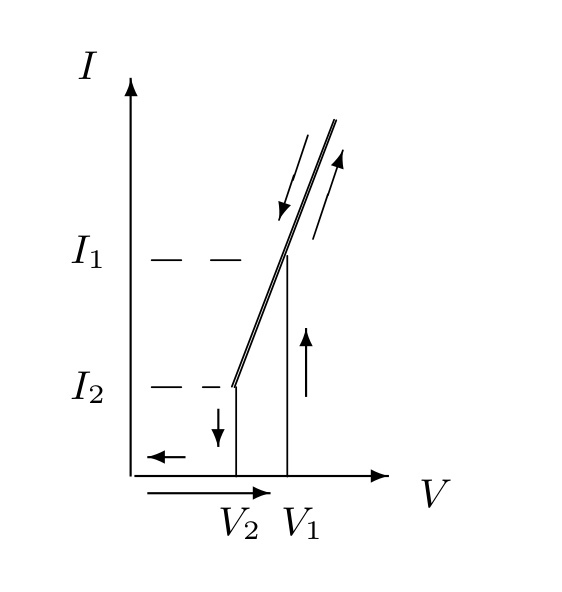
\includegraphics[scale=0.2]{pic1.jpg}
        \caption{Вольт-амперная характеристика стабилитрона с последовательно включенным резистором}
    \end{wrapfigure}
    В контуре, содержащем конденсатор и катушку индуктивности, электрическая энергия переходит в магнитную и обратно.

    Встречаются, однако, колебательные системы, содержащие всего один накопитель энергии.
    Рассмотрим в качестве примера электрическую цепь, содержащую конденсатор и сопротивление без самоиндукции. 
    Разряду, однако, можно придать периодический характер, возобновляя заряд конденсатора через постоянные промежутки времени. 
    Колебания вв этом случае являются совокупностью двух апериодических процессов~---~процесса зарядки конденсатора и процесса его разрядки. 
    Такие колебания называются релаксационными.


    В нашей установке роль "ключа", обеспечивающего попеременную зарядку и разрядку конденсатора, играет газоразрядный диод. 
    Зависимость тока от напряжения для газоразрядной лампы не подчиняется закону Ома и характеризуется рядом особенностей (рис. 1).
    При малых напряжениях лампа практически не пропускает тока. 

    \begin{wrapfigure}{l}{0.3\linewidth}
        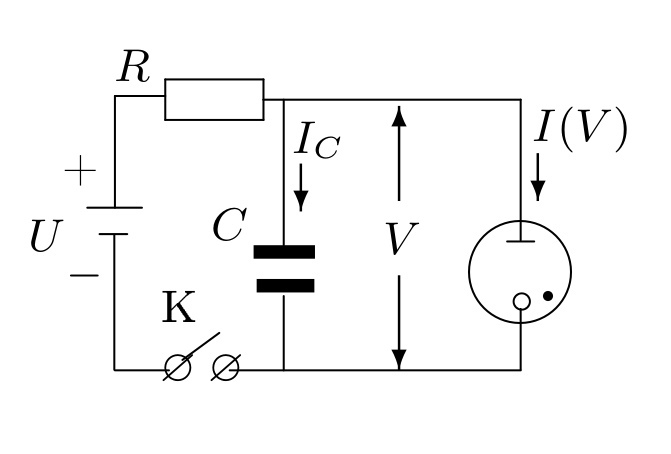
\includegraphics[scale=0.2]{pic2.jpg}
        \caption{Принципиальная схема релаксационного генератора}
    \end{wrapfigure}

    Ток в лампе возникает только в том случае, если разность потенциалов на ее электродах достигает напряжения зажигания $V_1$.
    При этом скачком устанавливается конечная сила тока $I_1$~---~в лампе возникает нормальный тлеющий заряд. 
    При дальнейшем незначительном увеличении напряжения сила тока заметно возрастает по закону, близкому к линейному.
    Нормальный тлеющий заряд~---~стабилизатор напряжения, отсюда второе название~---~стабиовольт.

    Если начать уменьшать напряжение на горящей лампе, то при напряжении, равном $V_1$, лампа еще не гаснет, и сила тока продолжает уменьшатся. 
    Лампа перестанет пропускать ток лишь при напряжении гашения $V_2$, которое обычно существенно меньше $V_1$.
    Сила тока при этом скачком падает от значения $I_2$ ($I_2 < I_1$) до нуля.

    Характеристика, изображенная на рис. 1, несколько идеализирована. 
    У реальной лампы зависимость $I\left(V\right)$ не вполне линейна.

    При $V > V1$ графики, соответствующие возрастанию и убыванию напряжения, не всегда совпадают. 
    Эти отличия, впрочем, носят второстепенный характер и для нашей задачи несущественны.

    \begin{wrapfigure}{l}{0.3\linewidth}
        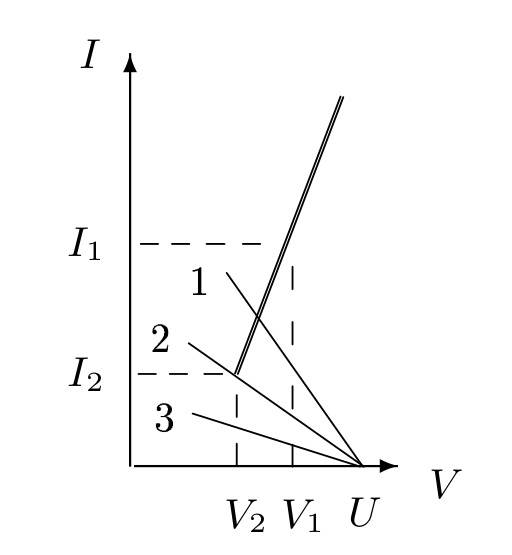
\includegraphics[scale=0.2]{pic3.jpg}
        \caption{Режимы работы релаксационного генератора}
    \end{wrapfigure}

    Рассмотрим схему релаксационного генератора, представленную на рис. 2. пусть напряжение батаери $U$ больше напряжения зажигания $V1$. В обозначениях, принятых на схеме, справедливо уравенение
    \begin{equation*}
        I_C + I\left(V\right) = \dfrac{U - V}{R}
    \end{equation*}
    или
    \begin{equation}
        C\dfrac{dV}{dt} + I\left(V\right) = \dfrac{U - V}{R}
    \end{equation}
    В стационарном режиме работы, когда напряжение $V$ на конденсаторе постоянно и $dV/dt = 0$, ток через лампу равен
    \begin{equation}
        I_{cт}=\dfrac{U - V}{R}
    \end{equation}

    Равенство (2) может быть представлено графически (рис. 3).

    При разных $R$ графики имею вид прямых, пересекающихся в точке $V = U, I = 0$.
    Область, где эти нагрузочные прямые пересекаются вольт-амперную характеристику лампы, соответствует стационарному режиму~---~при малых $R$ (прямая 1) лампа горит постоянно, колебания отсутствуют.
    Прямая 2, проходящая через точку $\left(I_2, V_2\right)$, соответствует критическому сопротивлению

    \begin{equation}
        R_{кр} = \dfrac{U - V_2}{I_2}
    \end{equation}

    При сопротивлении $R > R_{кр}$ нагрузочная прямая 3 не пересекает характеристику лампы, поэтому стационарный режим невозможен.
    В этом случае в системе устанавливаются колебания.

    Рассмотрим, как происходит колебательнй процесс. Пусть, в начале опыта ключ К разомкнут (рис. 2) и $V = 0$. 
    Замкнем ключ.
    Конденсатор $C$ начнет заряжаться через сопротивление $R$, напряжение на нем увеличивается (рис. 4).
    Как только оно достигент напряжения зажигания $V_1$, лампа начинает проводить ток, причем прохождение тока сопровождается разрядкой конденсатора.
    В самом деле батарея $U$, подключенная через большое сопротивление $R$, не может поддерживать необходимую для горения лампы величину тока.

    \begin{wrapfigure}{l}{0.3\linewidth}
        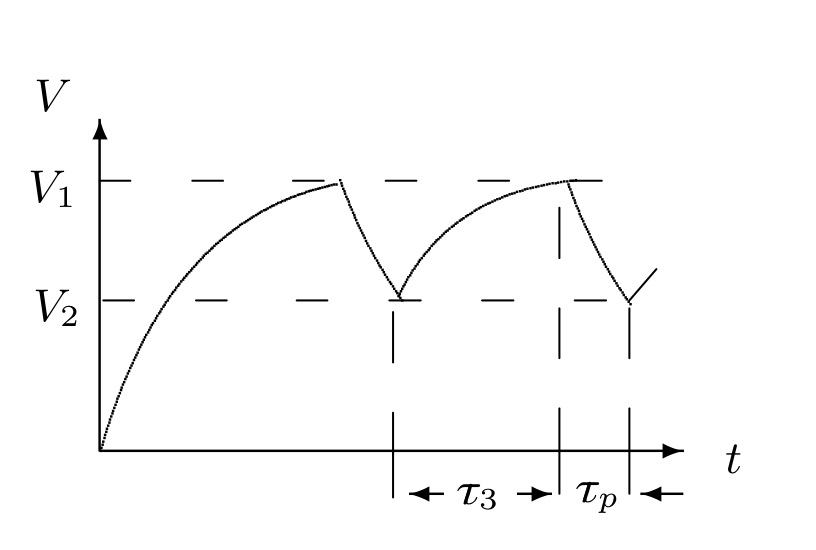
\includegraphics[scale=0.2]{pic4.jpg}
        \caption{Осциллограмма релаксационных колебаний}
    \end{wrapfigure}

    Во время горения лампы конденсатор разряжается, и когда напряжение на нем достигнет потенциала гашения, лампа перестанет проводить ток, а конденсатор вновь начнет заряжаться. 
    Возникают релаксационные колебания с амплитудой, равной $V1 - V2$.

    Рассчитаем период колебаний.
    Полное время одного периода колебаний $T$ состоит из суммы времени зарядки $\tau_з$ и времени разрядки $\tau_р$, но если сопротивление $R$ существенно превосходит сопротивление зажженой лампы, то $\tau_з \gg \tau_р$ и $T \approx \tau_з$ (этим случаем мы и ограничимся).
    
    Во время зарядки конденсатора лампа не горит ($I\left(V\right) = 0$), и уравенение (1) приобретает вид

    \begin{equation}
        R C \dfrac{dV}{dt} = U - V
    \end{equation}

    Будем отсчитывать время с момента гашения лампы, так что $V = V2$ при $t = 0$ (рис. 4).
    Решив уравнение (4), найдем

    \begin{equation}
        V = U - \left(U - V_2\right)\exp^{-t/RC}
    \end{equation}

    В момент зажигания $t = \tau_з, V = V_1$, поэтому

    \begin{equation}
        V_1 = U - \left(U - V_2\right)\exp^{-\tau_з/RC}
    \end{equation}

    Из уравнений (5) и (6) нетрудно найти период колебаний:

    \begin{equation}
        T \approx \tau_з = R C \ln{\dfrac{U - V_2}{U - V_1}}
    \end{equation}

    \mysec{Задание}
    
    \begin{wrapfigure}{l}{0.35\linewidth}
        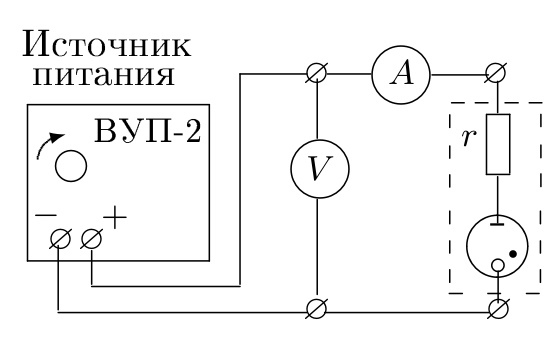
\includegraphics[scale=0.3]{pic5.jpg}
        \caption{Схема установки для изучения характеристик стабилитрона}
    \end{wrapfigure}
    В работе предлагается снять вольт-амперную характеристику стабилитрона и познакомиться с работой релаксационного генератора; определить критическое сопротивление, исследовать зависимость периода колебаний от сопротивления при фиксированной емкости и от емкости при фиксированном сопротивлении.\\\\\\\\\\\\

    \begin{center}
        Характеристика стабилитрона
    \end{center}

    \begin{enumerate}
        \item Соберем схему, изображенную на рис.5. Запишем величину $r$, указанную на панели лампы. $r = 5.4$ кОм
        \item Установим регулятор источника питания на минимум напряжения и включим источник в сеть.
        \item Снимем вольт-амперную характеристику стабилитрона с сопротивлением $r$ при возрастании и убывании напряжения. При этом как можно точнее определите потенциалы зжаигания и гашения $V_1$ и $V_2$ и соответствующие токи $I_1$ и $I_2$.\\
        
        \begin{tabular}{|c|c|c|c|c|c|c|c|}
            \hline
            \multicolumn{4}{|c|}{При возрастании} & \multicolumn{4}{|c|}{При убывании}\\ \hline
            $I$, мА & $U$, В & $I$, мА & $U$, В & $I$, мА & $U$, В & $I$, мА & $U$, В \\ \hline 
            3.37 & 91.25 & 5.47 & 103.33 & 6.26 & 106.48 & 3.8 & 93.55 \\ \hline
            3.72 & 93.25 & 5.78 & 105.12 & 5.92 & 105.1 & 3.5 & 92.02\\ \hline
            4.01 & 94.93 & 6.28 & 107.15 & 5.52 & 103.02 & 3.22 & 90.25 \\ \hline
            4.47 & 97.53 & 6.48 & 108.37 & 5.34 & 102.05 & 2.76 & 87.67\\ \hline
            4.76 & 99.15 &  &  & 4.87 & 99.25 & 2.26 & 84.97\\ \hline
            5.25 & 102.05 & & & 4.64 & 98.05 & 1.41 & 80.52\\ \hline
            & & & & & & 0 & 75.4 \\ \hline
        \end{tabular}

        \item $V_1 = 91.25$ В, $V_2 = 75.40$ В, $I_1 = 3.37$ мА, $I_2 = 0.43$ мА
        
        \begin{center}
            Осциллограммы релаксационных колебаний
        \end{center}

        \item Соберем релаксационный генератор согласно рис. 6
        \item Установим на магазине емкостей значение $C = 0.05$ мкФ, а на магазине сопротивлений $R = 900$ кОм
        \item Включим в сеть осциллограф, звуковой генератор и источник питания и Установим напряжение $U = 109.5$ В
        \item Подберем частоту развертки ЭО, при которой на экарне видна картина пилообразных колебаний (рис. 4). 
        \item Получив пилу на экране, оценим время зарядки и время разрядки $\tau_з = 60$ мс, $\tau_р = 5$ мс. Картина колебаний см. ниже\\
        
        \begin{figure}
            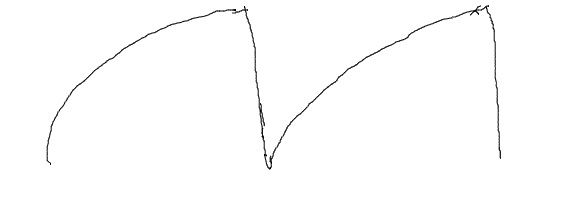
\includegraphics[scale=0.8]{pic6.jpg}
            \caption{Картина колебаний}
        \end{figure}

        \item Уменьшая сопротивление магазина, определим $R_{кр}$, при котором пропадают колебания и сравним его с величиной, рассчитаной по формуле (3).
        $R_{крт} = 0.8 * 10^5$ Ом, $R_{кр} = 1.4 * 10^5$ Ом
        
        \begin{figure}[!h]
            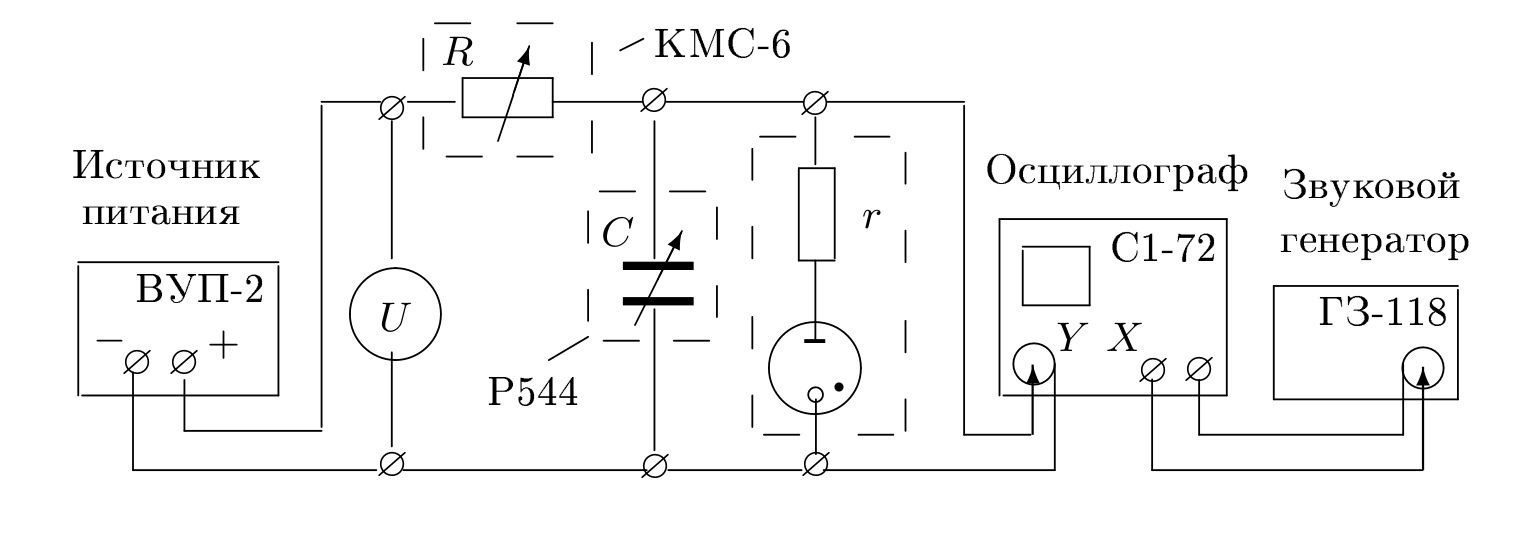
\includegraphics[scale=0.2]{pic7.jpg}
            \caption{Схема установки для исследования релаксационных колебаний}
        \end{figure}
        
        \newpage

        \begin{center}
            Фигуры Лиссажу 
        \end{center}

        \item Восстановим исходные параметры релаксационного генератора: $C = 5 \cdot 10^{-2}$ мкФ, $R = 900$ кОм, $U \approx 1.2 \cdot V_1$. Подадим сигнал с генератора на вход осциллографа. Меняя частоту ЗГ, получим на экране фигуры лиссажу без самопересечений, соответствующую отношению частот 1:1.
        \item Не меняя параметров релаксационного генератора, уменьшим частоту ЗГ вдвое (втрое) и получим фигуры Лиссажу при соотношении частот 2:1 (3:1). Кривые приведены ниже.
        
        \begin{figure}[!h]
            \begin{center}
                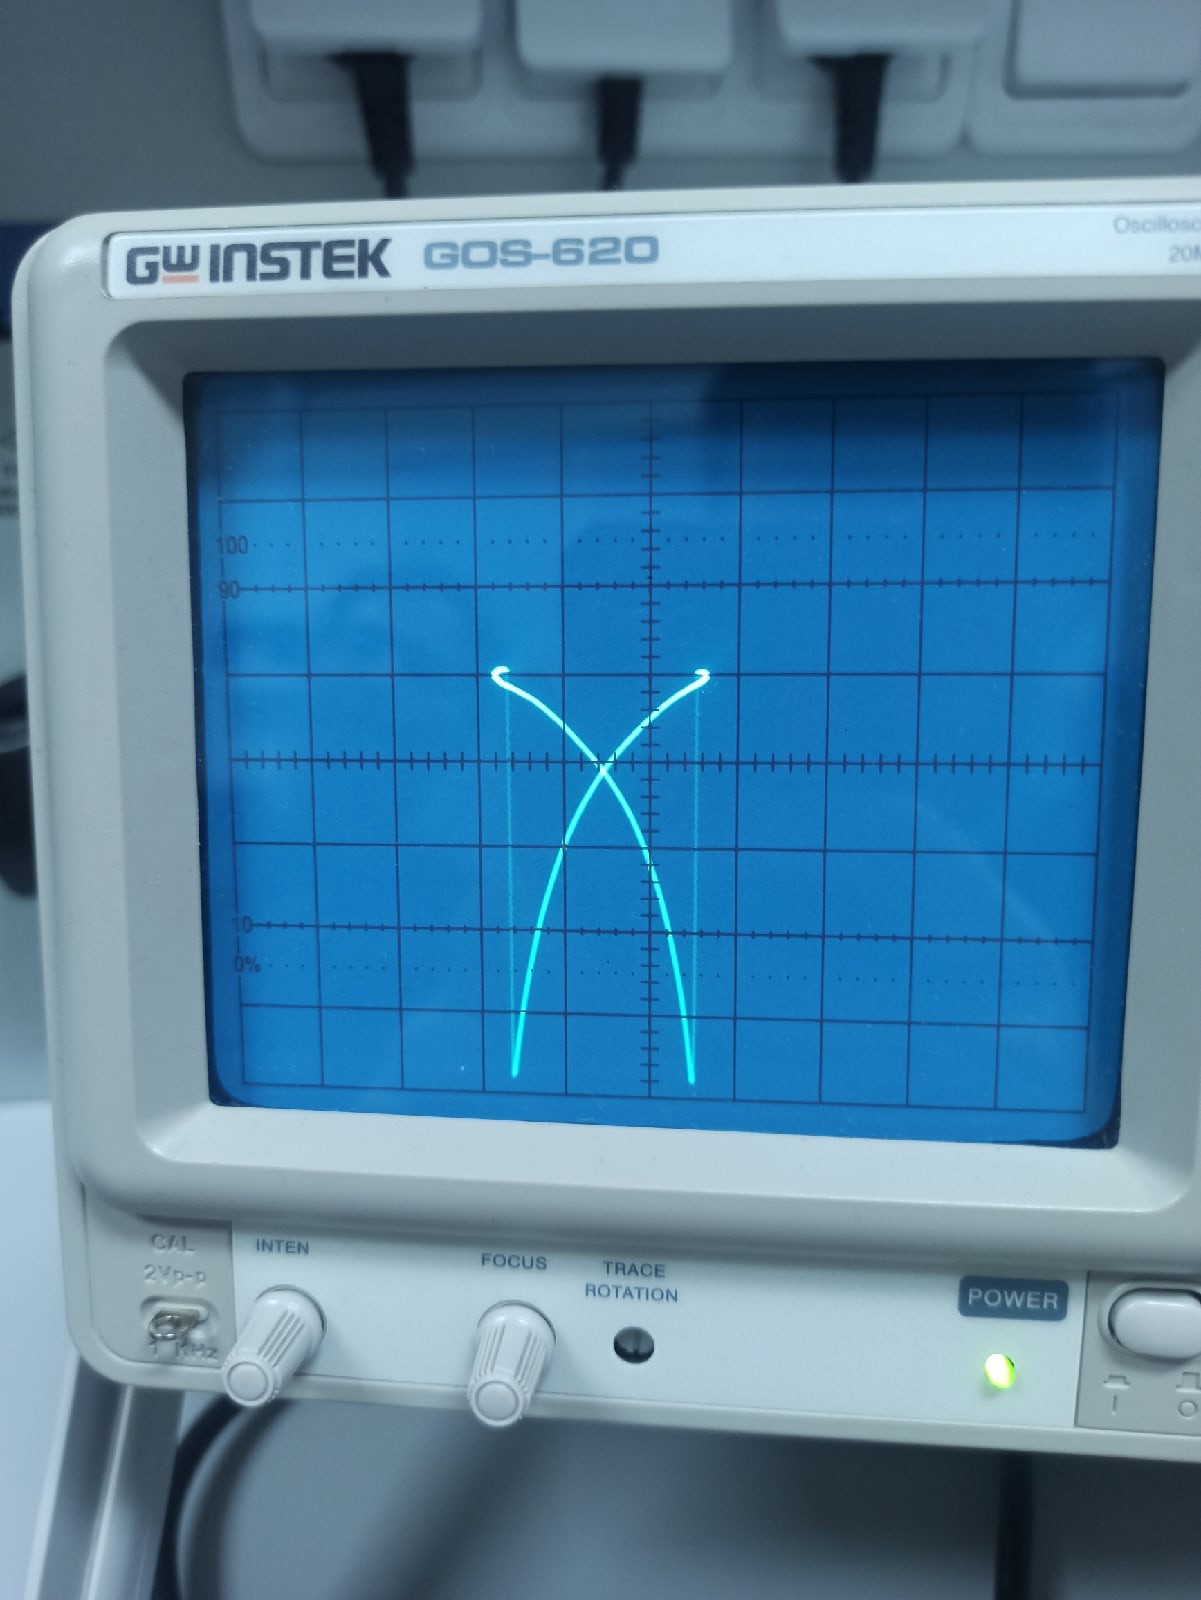
\includegraphics[scale=0.3]{pic8.jpg}
                \caption{Отношение частот 2:1}
            \end{center}
        \end{figure}

        \newpage

        \begin{figure}[!h]
            \begin{center}
                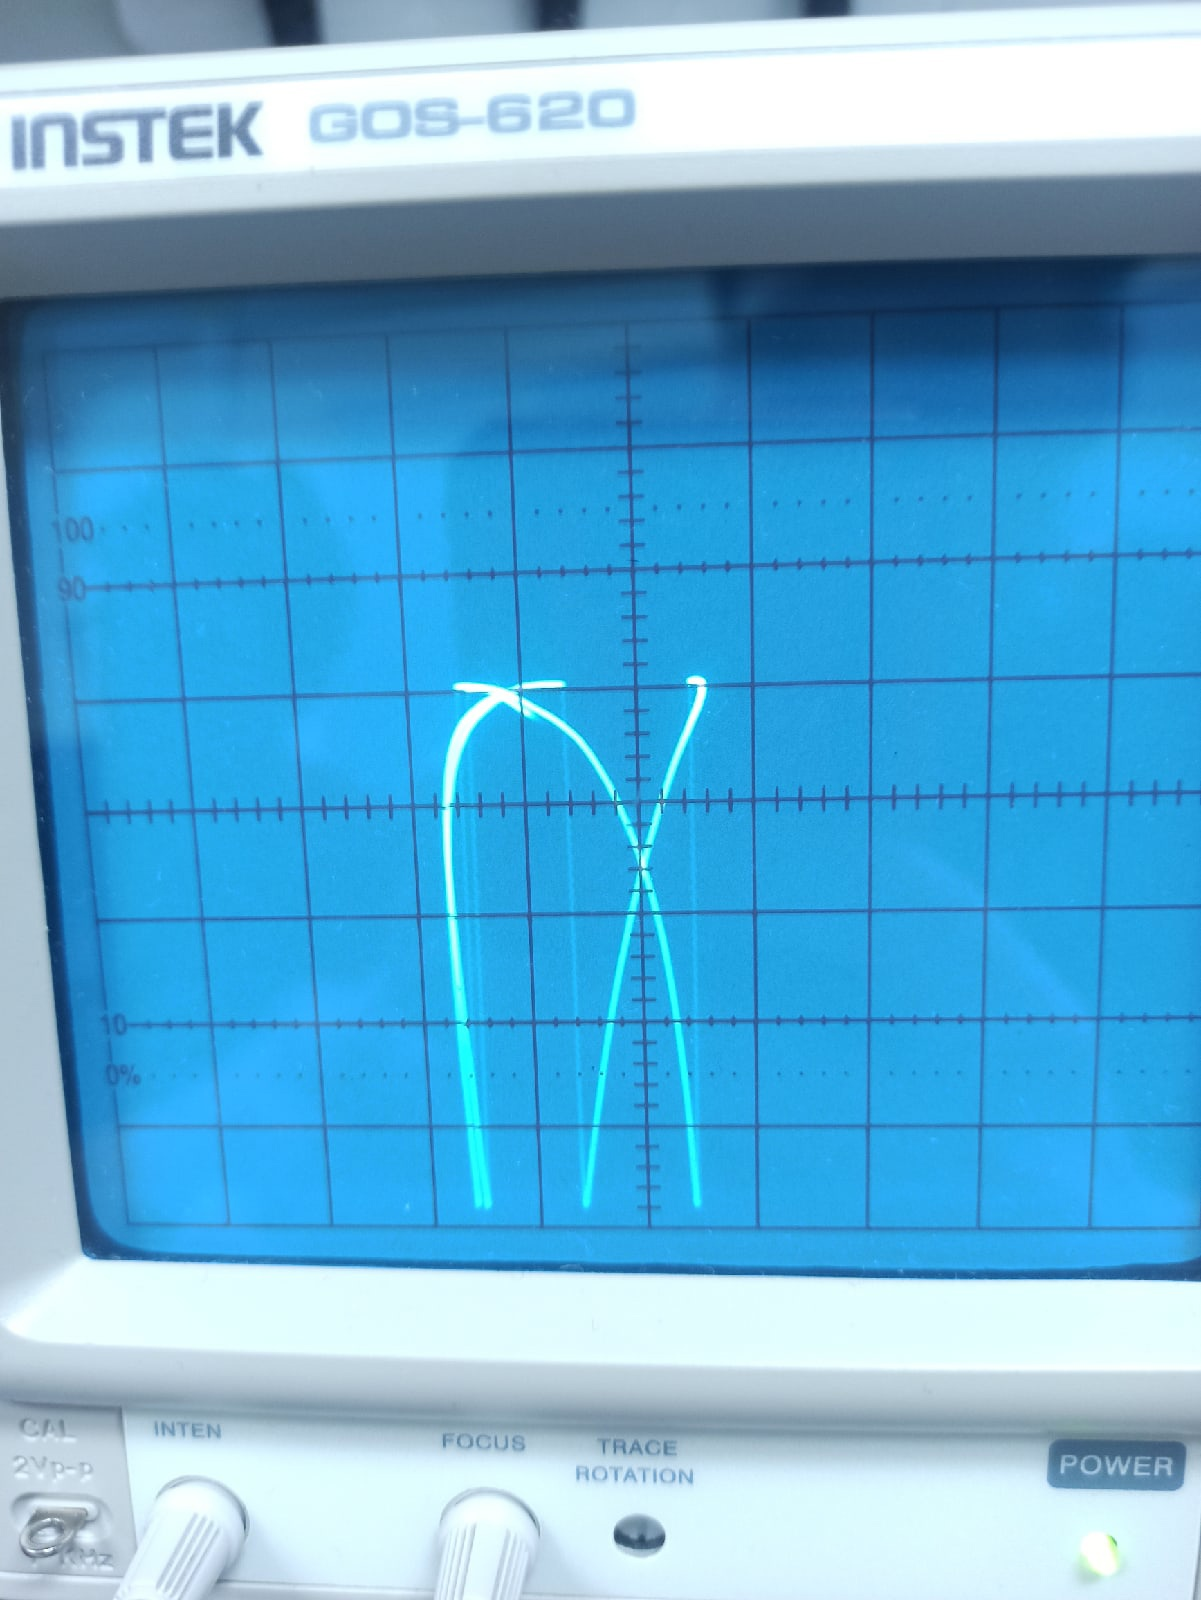
\includegraphics[scale=0.3]{pic9.jpg}
                \caption{Отношение частот 3:1}
            \end{center}
        \end{figure}

        \item При значении $R = 5.2 \cdot 10^5$ Ом снимем с помощью фигур Лиссажу 1:1 зависимость частоты колебаний $f$ от емкости $C$, меняя величину емкости. Напряжение поддерживаем постоянным, $U = 109.5$ В (таблицу см. ниже)

        \item Проведем серию измерений $f = f\left(R\right)$ при постоянной емкости $C = 0.05$ мкФ, меняя величину $R$ от максимального значения до критического.
        
        \begin{tabular}{|c|c|c|c|c|c|}
            \hline
            \multicolumn{2}{|c|}{$R = 5.2 \cdot 10^5$ Ом} & \multicolumn{2}{|c|}{$C = 0.05$ мкФ} & \multicolumn{2}{|c|}{$C = 0.05$ мкФ}\\ \hline
            $f$, Гц & $C$, мкФ & $f$, Гц & $R, 10^5$ Ом & $f$, Гц & $R, 10^5$ Ом \\ \hline
            150 & 0.01 & 17 & 9 & 39.5 & 4\\ \hline
            75 & 0.02 & 19 & 8 & 53 & 3\\ \hline
            50 & 0.03 & 22 & 7 & 78.2 & 2\\ \hline
            37 & 0.04 & 25.7 & 6 & & \\ \hline
            30 & 0.05 & 31 & 5 & & \\ \hline
        \end{tabular}
    \end{enumerate}

    \begin{center}
        Обработка результатов
    \end{center}

    \begin{enumerate}
        \item Построим графики $I = f\left(V\right)$ для системы, состоящей из стабилитрона и дополнительного сопротивления $r$ (по результатам измерений) и для стабилитрона без сопротивления (вычитая падения напряжения на сопротивлении при каждом токе).
        
        \begin{figure}[!h]
            \begin{center}
                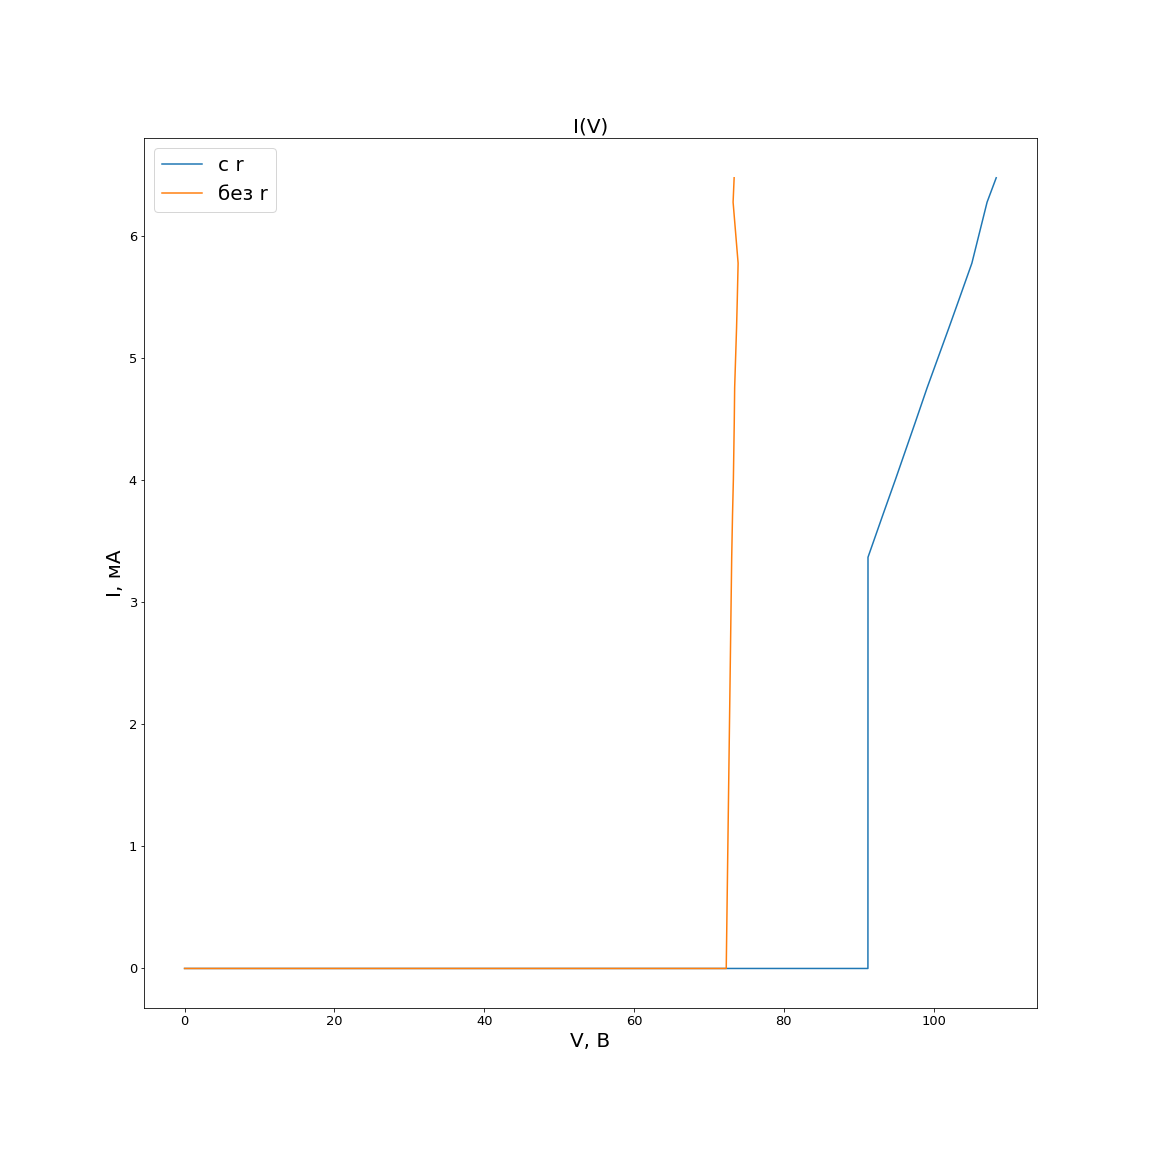
\includegraphics[scale=0.4]{graph1.png}
                \caption{График для пункта 1 обработки результатов}
            \end{center}
        \end{figure}

        \item Рассчитаем экспериментальные и теоретические значения периодов, построим графики $T_{эскп} = f\left(C\right)$ и $T_{теор} = f\left(C\right)$. На другом листе построим графики зависимостей периодов от $R$.
        \newpage
        \begin{figure}[!h]
            \begin{center}
                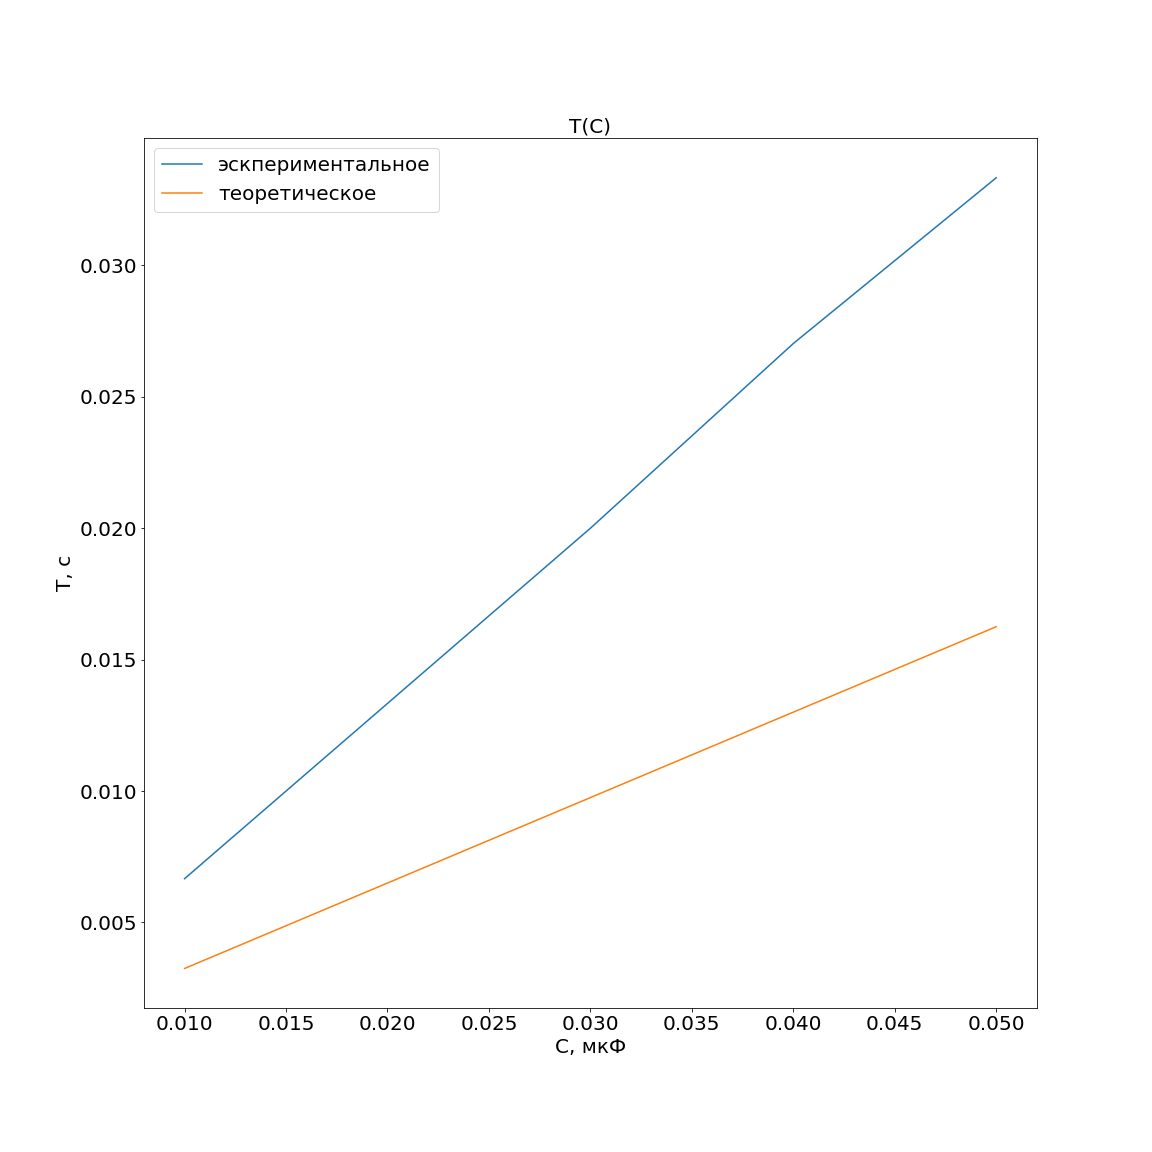
\includegraphics[scale=0.3]{graph2.png}
                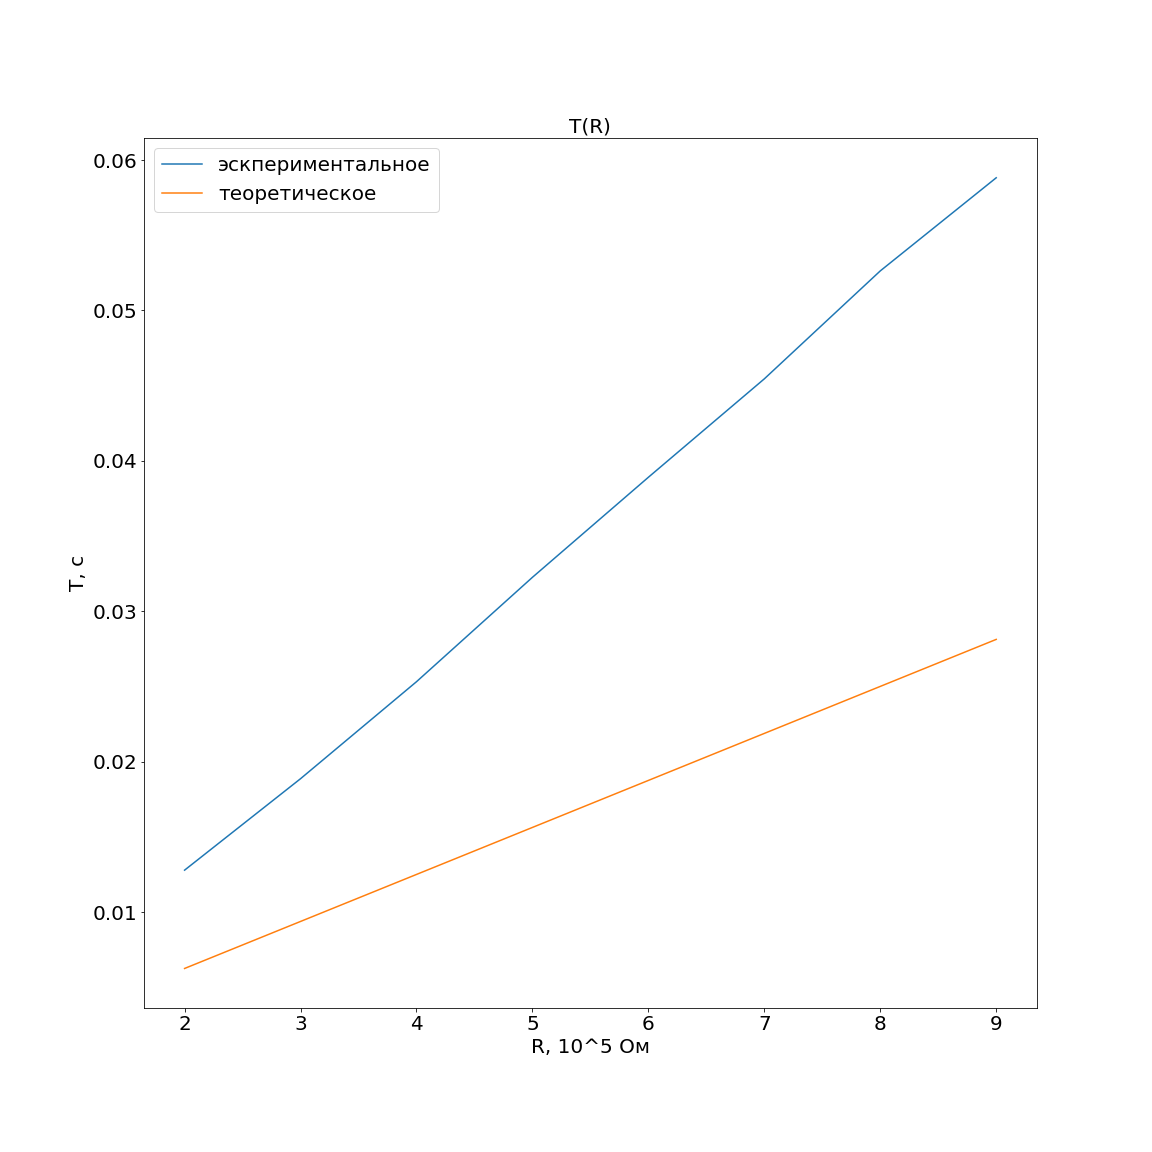
\includegraphics[scale=0.3]{graph3.png}
                \caption{Графики $T(C)$ и $T(R)$ для пункта 2 обработки результатов}
            \end{center}
        \end{figure}

    \end{enumerate}
\end{document}